\documentclass[runningheads]{llncs}
\usepackage{polski}
\usepackage[utf8x]{inputenc}
\usepackage{graphicx}
\usepackage[polish]{babel}
%\usepackage{geometry}
\usepackage{hyperref}
\usepackage{amsmath}
\usepackage[numbers]{natbib}
\usepackage{rotating}
\usepackage{verbatim}
\pagestyle{headings}  
\addtocmark{Algorytm ewolucyjny z funkcją celu aproksymowaną modelem 
zastępczym} 
%
%
%-%-% POCZĄTEK ARTYKUŁU
%
\title{Algorytm ewolucyjny z funkcją celu aproksymowaną modelem zastępczym}
% 
\titlerunning{Algorytm ewolucyjny z funkcją celu aproksymowaną modelem 
zastępczym}   
%
\author{Piotr Jarosik\\Marek Lewandowski}
%
\authorrunning{Piotr Jarosik, Marek Lewandowski} 
%
%
\institute{Wydział Elektroniki i~Technik Informacyjnych\\
Politechnika Warszawska\\
\email{P.Jarosik@stud.elka.pw.edu.pl\\
	M.M.Lewandowski@stud.elka.pw.edu.pl}}

\begin{document}
\maketitle

\section{Zadanie}
Implementacja i testowanie algorytmu ewolucyjnego, w którym funkcja celu 
jest aproksymowana modelem zastępczym. Na ten model proponuję IBHM, MLP lub 
model jądrowy.

\section{Interpretacja}

Celem zadania było zaimplementowanie i przetestowanie algorytmu ewolucyjnego, 
który do optymalizacji wykorzystuje model zastępczy zamiast rzeczywistej 
funkcji celu (która może być \emph{kosztowna obliczeniowo}). Rozwiązanie składa 
się z następujących kroków:
\begin{enumerate}
 \item Budowany jest aproksymator dla pewnej liczby punktów obliczonych dla 
rzeczywistej funkcji celu;
 \item Zbudowany w poprzednim punkcie aproksymator jest wykorzystywany do 
zadania optymalizacji -- poszukiwane jest optimum zbudowanego aproksymatora;
 \item Na podstawie wyników dobierany zostanie kolejny zbiór punktów, dla 
których następnie liczone są wartości rzeczywistej funkcji celu.
\end{enumerate}

Kroki te wykonywane są w pętli tak długo, aż osiągnięty zostanie odpowiedni 
poziom dokładności (zdefiniowany w kolejnych punktach) lub pewna ustalona 
maksymalna liczba iteracji.

\section{Opracowane rozwiązanie}

Rozwiązanie zostało opracowane zgodnie z podaną interpretacją projektu. 
Przyjęto następujące założenia:
\begin{itemize}
 \item jako model zastępczy zastosowano wielowarstwowy perceptron (MLP);
 \item optymalizatorem funkcji celu jest algorytm ewolucyjny (zgodnie z treścią 
zadania).
\end{itemize}
Uszczegółowienia wymaga jeszcze sposób doboru punktów w pierwszej i kolejnych 
iteracjach opracowanego algorytmu. 

W pierwszej iteracji budowane jest \emph{ogólne spojrzenie na rzeczywistą 
funkcję celu} -- aproksymator jest budowany na podstawie punktów wylosowanych z 
dziedziny z rozkładem jednostajnym. Pozwala to 
na określenie potencjalnych miejsc, gdzie być może znajduje się optimum 
rzeczywistej funkcji celu -- dokonywana jest \textbf{eksploracja} dziedziny. 
Jako granice rozkładu jednostajnego przyjęto ograniczenia kostki 
nałożone na daną funkcję (badana jest cała dopuszczalna dziedzina).

W kolejnych iteracjach szczegółowo badane są miejsca, w których być może 
znajduje się optimum globalne funkcji celu -- aproksymator budowany jest na 
podstawie sumy zbioru punktów wylosowanych do tej pory oraz zbioru punktów 
wylosowanych w otoczeniu optimum globalnego znalezionego w poprzedniej 
iteracji. W ten sposób szczegółowo zbadany został obszar potencjalnie 
zawierający optimum globalne rzeczywistej funkcji (\textbf{eksploatacja}) - 
dzięki temu możliwa jest korekta otrzymanego optimum i być może zmiana 
obszaru dziedziny, z którego będą losowane punkty w kolejnych iteracjach (gdy 
np. dotychczas znalezione optimum globalne, po zwiększeniu liczby punktów w 
jego otoczeniu, okaże się być tylko optimum lokalnym). Punkty w trakcie 
eksploatacji są losowane z rozkładem normalnym o wartości oczekiwanej równej 
znalezionemu optimum i macierzy kowariancji dobranej do ograniczeń rzeczywistej 
funkcji celu (tak, aby poszukiwanie było dokonywane głównie wokół wartości 
oczekiwanej, z uwzględnieniem punktów możliwych wokół znalezionego optimum).

Algorytm kończy działanie, gdy:
\begin{itemize}
 \item osiągnięto dobrą aproksymację rzeczywistej funkcji celu -- błąd 
średniokwadratowy nie uległ poprawie przez pewną ustaloną liczbę iteracji;
 \item przekroczono maksymalną liczbę iteracji.
\end{itemize}

Poniżej przedstawiono szczegóły zaimplementowanego algorytmu ewolucyjnego oraz 
perceptronu wielowarstwowego.

\subsection{Algorytm ewolucyjny}

Algorytm ewolucyjny został zaimplementowany zgodnie ze schematem 
zaprezentowanym w \cite{arabas}. Unkonkretyzowania 
wymagają jednak poszczególne operatory, inicjacja populacji oraz kryterium 
zatrzymania. 

\subsubsection{Inicjacja}

Populacja początkowa algorytmu ewolucyjnego wybierana jest z rozkładem 
normalnym o niskiej wariancji (w ramach projektu przyjęto arbitralnie 
wartość $0.1$) wokół punktu początkowego. Punkt początkowy stanowi parametr 
algorytmu \footnote{W rzeczywistości punkt początkowy często jest podawany wraz 
z funkcją celu. Tak jest w przypadku benchmarka BBOB13 -- jednym z 
parametrów wejściowych algorytmu optymalizacji jest punkt początkowy 
proponowany przez benchmark).}

\subsubsection{Selekcja}
W ramach projektu przyjęto \textbf{selekcję turniejową}: w \emph{szranki} 
losowane są punkty z rozkładem jednostajnym z obecnego stanu populacji. 
Następnie reprodukcji (selekcji) podlega najlepszy punkt ze szranki (tj. o 
największej wartości funkcji celu).

\subsubsection{Krzyżowanie}
Opracowany projekt wykorzystuje \textbf{krzyżowanie równomierne}, tj. nowy 
punkt (po skrzyżowaniu) definiowany jest jako:
\begin{equation}
 y = wx_1 + (1-w)x_2
\end{equation}
przy czym $w$ jest wektorem binarnym z jednakowym prawdopodobieństwem jedynek i 
zer. Krzyżowaniu podlegają dokładnie dwa punkty. Krzyżowanie dokonywane jest 
tylko, gdy pewna ustalona zmienna losowa o rozkładzie jednostajnym przekroczy 
wybrany próg -- prawdopodobieństwo krzyżowania. W ramach projektu próg ten 
został ustalony jako $0.5$.

\subsubsection{Mutacja}
Mutacja dokonywana jest z rozkładem normalnym z ustaloną (sparametryzowaną) 
wartością macierzy kowariancji.

\subsubsection{Sukcesja}
W ramach projektu przyjęto \textbf{sukcesję elitarną} -- nowa populacja składa 
się z $\mu$ najlepszych osobników z nowej populacji (wyniku zastosowanych 
powyżej operacji) oraz $k$ najlepszych poprzedniej populacji. W przypadku 
zrealizowanego projektu przyjęto arbitralnie $k=1$.

\subsection{Kryterium zatrzymania}
Jako kryterium zatrzymania algorytmu przyjęto:
\begin{itemize}
 \item brak poprawy jakości rozwiązania przez $\tau$ ostatnich iteracji, tj.
\begin{equation}
 \Phi(X(t-\tau))-\Phi(X(t)) \le \epsilon
\end{equation}
gdzie $\Phi$ -- funkcja celu, $X(t)$ -- najlepszy osobnik znaleziony do chwili 
$t$, $\epsilon$ i $\tau$ -- parametry algorytmu (w ramach projektu przyjęto 
wartości odpowiednio $10$ oraz $0.1$.
\end{itemize}

\subsection{Perceptron wielowarstwowy}
\label{sec:aprox}
Zgodnie z założeniami użyto perceptronu wielowarstwowego do budowy modelu 
zastępczego - aproksymatora funkcji celu. W tym celu, w ramach projektu 
skorzystano z gotowego pakietu języka R \verb neuralnet , który pozwala na 
budowę sieci neuronowej o dowolnej liczbie warstw ukrytych, liczbie ukrytych 
neuronów, wybór funkcji aktywacji, wybór metody optymalizacji i innych 
parametrów.

Użyto sieci o następujących parametrach:
\begin{itemize}
\item sieć składa się z 3 warstw, w tym jednej warstwy ukrytej,
\item sieć posiada tylko jeden neuron wyjściowy,
\item wyjście sieci jest liniowe,
\item funkcja aktywacji to tangens hiperboliczny,
\item miarą błędu na zbiorze trenującym jest błąd średniokwadratowy,
\item metoda optymalizacji to RPROP+
\item rozmiar wejścia sieci jest parametryzowany w zależności od aktualnie badanej funkcji i jej wymiaru,
\item liczba neuronów warstwy ukrytej jest parametryzowana podczas badań.
\end{itemize}

Ponadto zastosowano metodę normalizacji danych przed rozpoczęciem trenowania 
sieci w celu przyspieszenia algorytmu. Podczas predykcji dane są normalizowane, a wynik denormalizowany.

\subsection{Proces normalizacji}
Próbkę danych $x$ normalizuje się zgodnie ze wzorem:

$x_{norm}=\frac{x - m}{sd}$

gdzie:	$m$ - wartość oczekiwana $x$, $sd$ - standardowe odchylenie $x$.
Wzór podano dla formy wektorowej.

\section{Eksperymenty}
Celem eksperymentów jest zbadanie, jak optymalizacja z wykorzystaniem modelu 
zastępczego wpływa na jakość otrzymywanego rozwiązania. Eksperymenty 
przeprowadzono przy użyciu benchmarku BBOB13. Testy zostały przeprowadzone dla 
funkcji z zakresu $1-24$ dla wymiarów $5D$ oraz $20D$. 

Mając na uwadze charakter problemu, czyli wysoki koszt ewaluacji rzeczywistej 
funkcji, ważnym parametrem oceny rozwiązania jest maksymalna liczba ewaluacji 
funkcji celu FEsmax(fixed cost). Głównym punktem badań była więc analiza liczby 
ewaluacji funkcji niezbędnej do osiągnięcia pewnego poziomu jakości 
rozwiązania. W tym celu, do prezentacji wyników posłużono się łączną 
dystrybuantą empiryczną (ECDF) dla rozkładów liczby ewaluacji funkcji przy 
ustalonym poziomie błędu oraz łączną dystrybuantą empiryczną dla rozkładu 
najlepszych osiągniętych poziomów błędu. Zamieszczone wykresy zostały 
wygenerowane przy użyciu skryptu w języku python opracowanego przez autorów 
benchmarku BBOB13.

Aby mieć pewien punkt odniesienia, opracowane rozwiązanie porównano z 
samym algorytmem ewolucyjnym, który stanowi element opracowanego rozwiązania. 
Parametry, których zmiany zostały badane to: rozmiar utrzymywanej populacji 
($\mu$), rozmiar reprodukowanej populacji ($\lambda$), maksymalna liczba 
iteracji opracowanego algorytmu. Ponadto sprawdzono, jak zmiana liczby 
neuronów na warstwie ukrytej wpływa na jakość opracowanego rozwiązania.

\section{Wyniki}
\newcommand{\rot}[2][2.5]{
  \hspace*{-3.5\baselineskip}%
  \begin{rotate}{90}\hspace{#1em}#2
\end{rotate}}
  
Poniżej przedstawiono wykresy ECDF otrzymane w procedurze eksperymentalnej. Po 
lewej stronie każdej kolumny umieszczone są dystrybuanty rozkładów w dziedzinie 
liczby ewaluacji funkcji celu, zaś w po prawej -- dystrybuanta rozkładu jakości 
(odległości od optimum) dla otrzymywanych wyników. Eksperymenty zostały 
wykonane dla budżetu równego 100.
\newpage  
\subsection{Algorytm ewolucyjny bez modelu zastępczego}
Parametry:
\begin{itemize}
 \item rozmiar utrzymywanej populacji $P^t$: $\mu=100$
 \item rozmiar reprodukowanej populacji $O^t$: $\lambda=100$
 \item maksymalna liczba iteracji algorytmu ewolucyjnego: $10000$
\end{itemize}
\begin{figure*}
\begin{tabular}{l@{\hspace*{-0.025\textwidth}}l@{\hspace*{-0.00\textwidth}}|l@{
\hspace*{-0.025\textwidth}}l}
\multicolumn{2}{c}{$D=5$} & \multicolumn{2}{c}{$D=20$}\\[-0.5ex]
\rot{separable}
\includegraphics[width=0.268\textwidth,trim=0 0 0 13mm, 
clip]{ppdata_ev/pprldistr_05D_separ} &
\includegraphics[width=0.2362\textwidth,trim=2.40cm 0 0 13mm, 
clip]{ppdata_ev/ppfvdistr_05D_separ} &
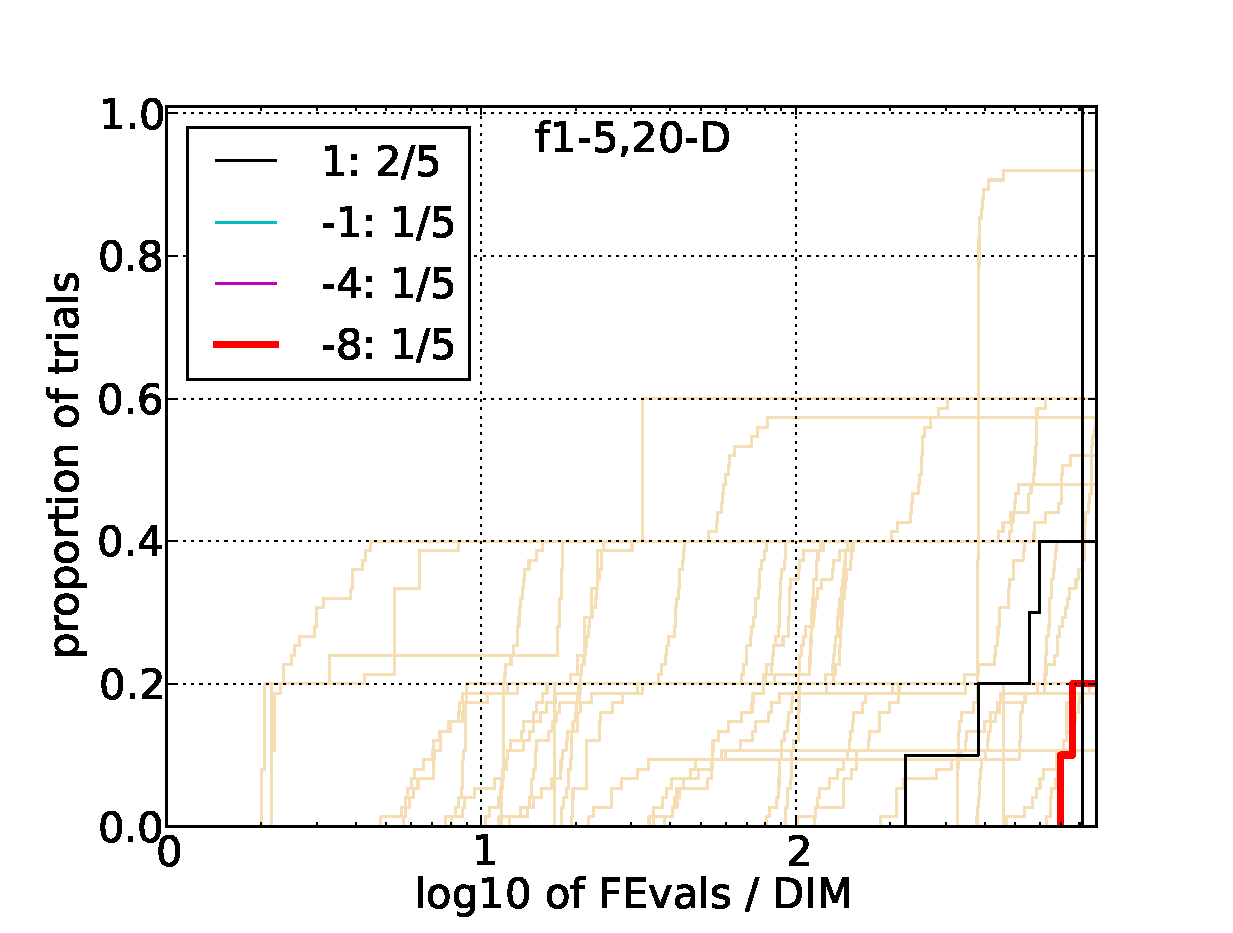
\includegraphics[width=0.268\textwidth,trim=0 0 0 13mm, 
clip]{ppdata_ev/pprldistr_20D_separ} &
\includegraphics[width=0.2362\textwidth,trim=2.40cm 0 0 13mm, 
clip]{ppdata_ev/ppfvdistr_20D_separ} \\[-2ex]
\rot[1]{moderate}
\includegraphics[width=0.268\textwidth,trim=0 0 0 13mm, 
clip]{ppdata_ev/pprldistr_05D_lcond} &
\includegraphics[width=0.2362\textwidth,trim=2.40cm 0 0 13mm, 
clip]{ppdata_ev/ppfvdistr_05D_lcond} &
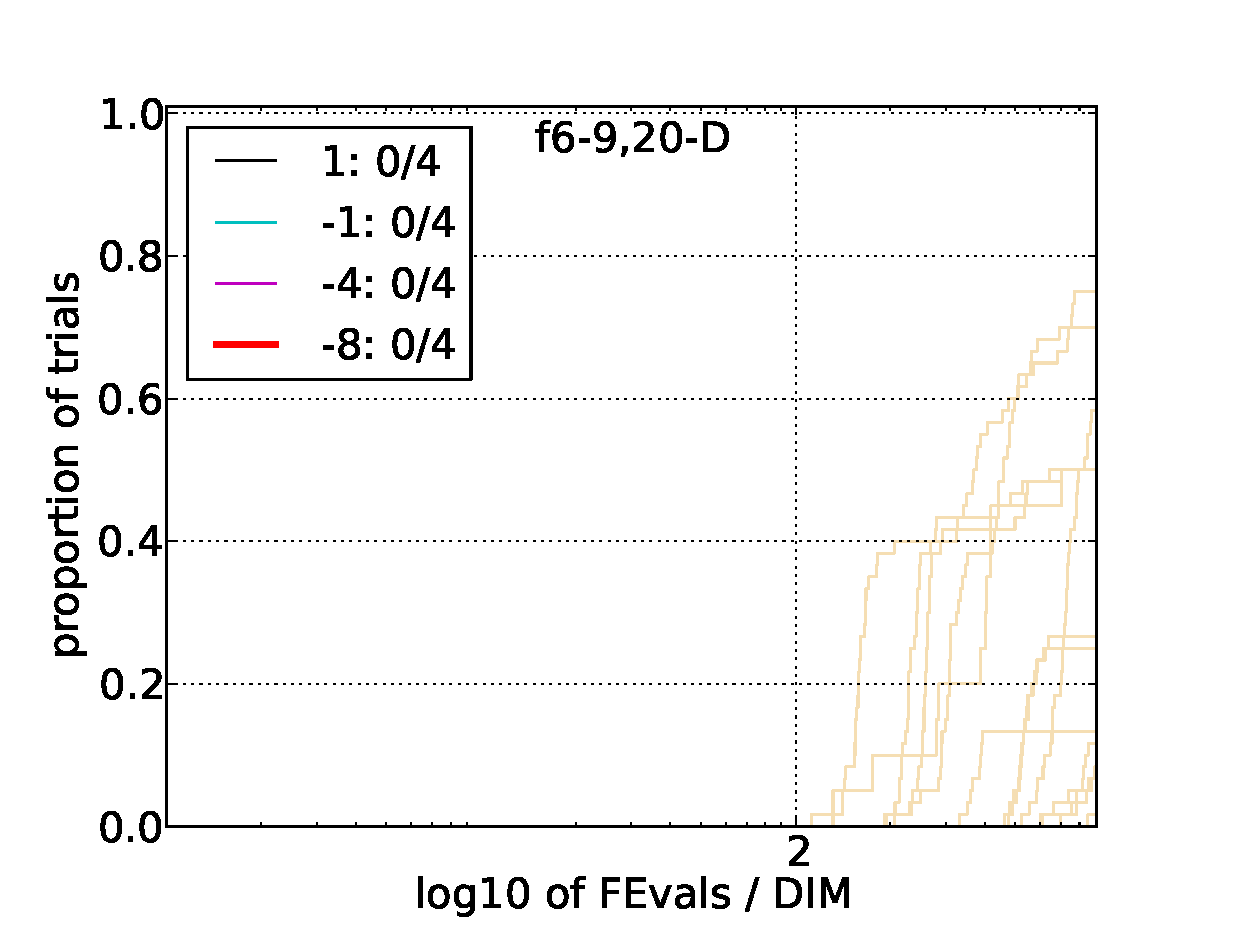
\includegraphics[width=0.268\textwidth,trim=0 0 0 13mm, 
clip]{ppdata_ev/pprldistr_20D_lcond} &
\includegraphics[width=0.2362\textwidth,trim=2.40cm 0 0 13mm, 
clip]{ppdata_ev/ppfvdistr_20D_lcond} \\[-2ex]
\rot[1.3]{ill-cond.}
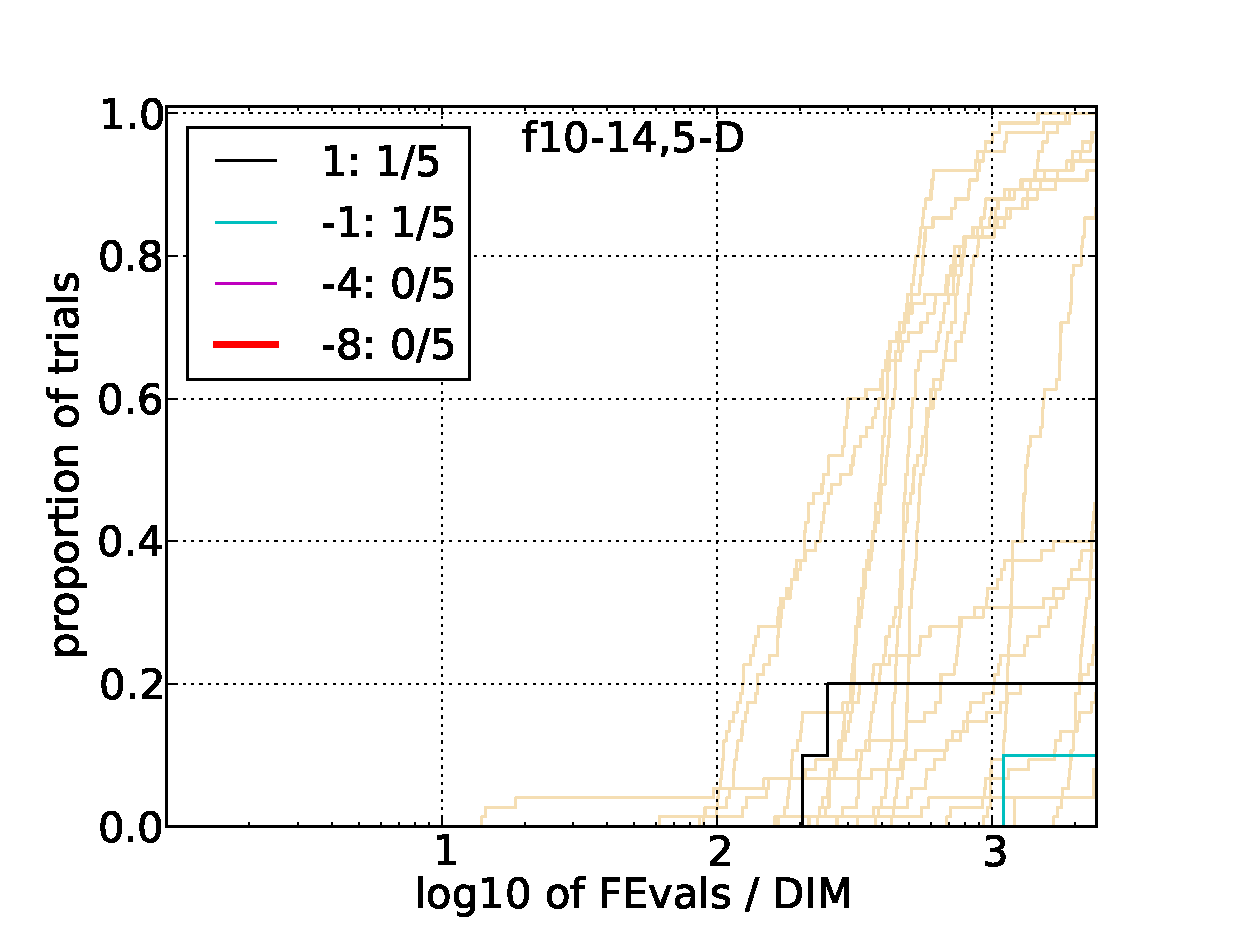
\includegraphics[width=0.268\textwidth,trim=0 0 0 13mm, 
clip]{ppdata_ev/pprldistr_05D_hcond} &
\includegraphics[width=0.2362\textwidth,trim=2.40cm 0 0 13mm, 
clip]{ppdata_ev/ppfvdistr_05D_hcond} &
\includegraphics[width=0.268\textwidth,trim=0 0 0 13mm, 
clip]{ppdata_ev/pprldistr_20D_hcond} &
\includegraphics[width=0.2362\textwidth,trim=2.40cm 0 0 13mm, 
clip]{ppdata_ev/ppfvdistr_20D_hcond} \\[-2ex]
\rot[1.6]{multi-modal}
\includegraphics[width=0.268\textwidth,trim=0 0 0 13mm, 
clip]{ppdata_ev/pprldistr_05D_multi} &
\includegraphics[width=0.2362\textwidth,trim=2.40cm 0 0 13mm, 
clip]{ppdata_ev/ppfvdistr_05D_multi} &
\includegraphics[width=0.268\textwidth,trim=0 0 0 13mm, 
clip]{ppdata_ev/pprldistr_20D_multi} &
\includegraphics[width=0.2362\textwidth,trim=2.40cm 0 0 13mm, 
clip]{ppdata_ev/ppfvdistr_20D_multi} \\[-2ex]
\rot[1.0]{weak struct}
\includegraphics[width=0.268\textwidth,trim=0 0 0 13mm, 
clip]{ppdata_ev/pprldistr_05D_mult2} &
\includegraphics[width=0.2362\textwidth,trim=2.40cm 0 0 13mm, 
clip]{ppdata_ev/ppfvdistr_05D_mult2} &
\includegraphics[width=0.268\textwidth,trim=0 0 0 13mm, 
clip]{ppdata_ev/pprldistr_20D_mult2} &
\includegraphics[width=0.2362\textwidth,trim=2.40cm 0 0 13mm, 
clip]{ppdata_ev/ppfvdistr_20D_mult2}\\[-2ex]
\rot{all}
\includegraphics[width=0.268\textwidth,trim=0 0 0 13mm, 
clip]{ppdata_ev/pprldistr_05D_noiselessall} &
\includegraphics[width=0.2362\textwidth,trim=2.40cm 0 0 13mm, 
clip]{ppdata_ev/ppfvdistr_05D_noiselessall} &
\includegraphics[width=0.268\textwidth,trim=0 0 0 13mm, 
clip]{ppdata_ev/pprldistr_20D_noiselessall} &
\includegraphics[width=0.2362\textwidth,trim=2.40cm 0 0 13mm, 
clip]{ppdata_ev/ppfvdistr_20D_noiselessall}
\vspace*{-0.5ex}
\end{tabular}
\caption{Wykresy ECDF dla algorytmu ewolucyjnego bez modelu zastępczego.}
\end{figure*}
\newpage
\subsection{Algorytm ewolucyjny z wykorzystaniem modelu zastępczego}
Parametry:
\begin{itemize}
 \item rozmiar utrzymywanej populacji $P^t$: $\mu=100$
 \item rozmiar reprodukowanej populacji $O^t$: $\lambda=100$
 \item maksymalna liczba iteracji algorytmu ewolucyjnego: $10000$
 \item liczba neuronów w warstwie ukrytej: $10$
\end{itemize}
\begin{figure*}[!h]
\begin{tabular}{l@{\hspace*{-0.025\textwidth}}l@{\hspace*{-0.00\textwidth}}|l@{
\hspace*{-0.025\textwidth}}l}
\multicolumn{2}{c}{$D=5$} & \multicolumn{2}{c}{$D=20$}\\[-0.5ex]
\rot{separable}
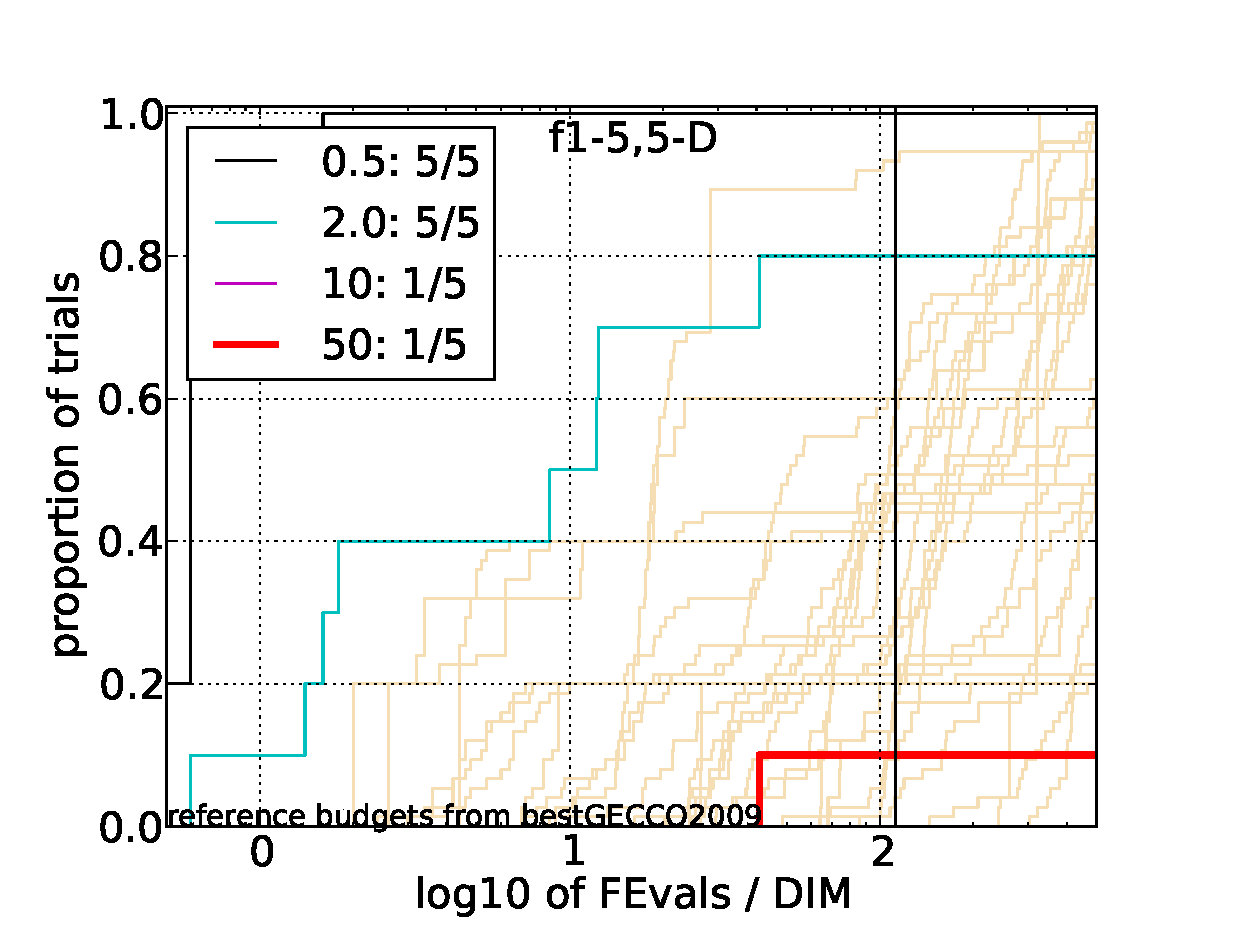
\includegraphics[width=0.268\textwidth,trim=0 0 0 13mm, 
clip]{ppdata_normal/pprldistr_05D_separ} &
\includegraphics[width=0.2362\textwidth,trim=2.40cm 0 0 13mm, 
clip]{ppdata_normal/ppfvdistr_05D_separ} &
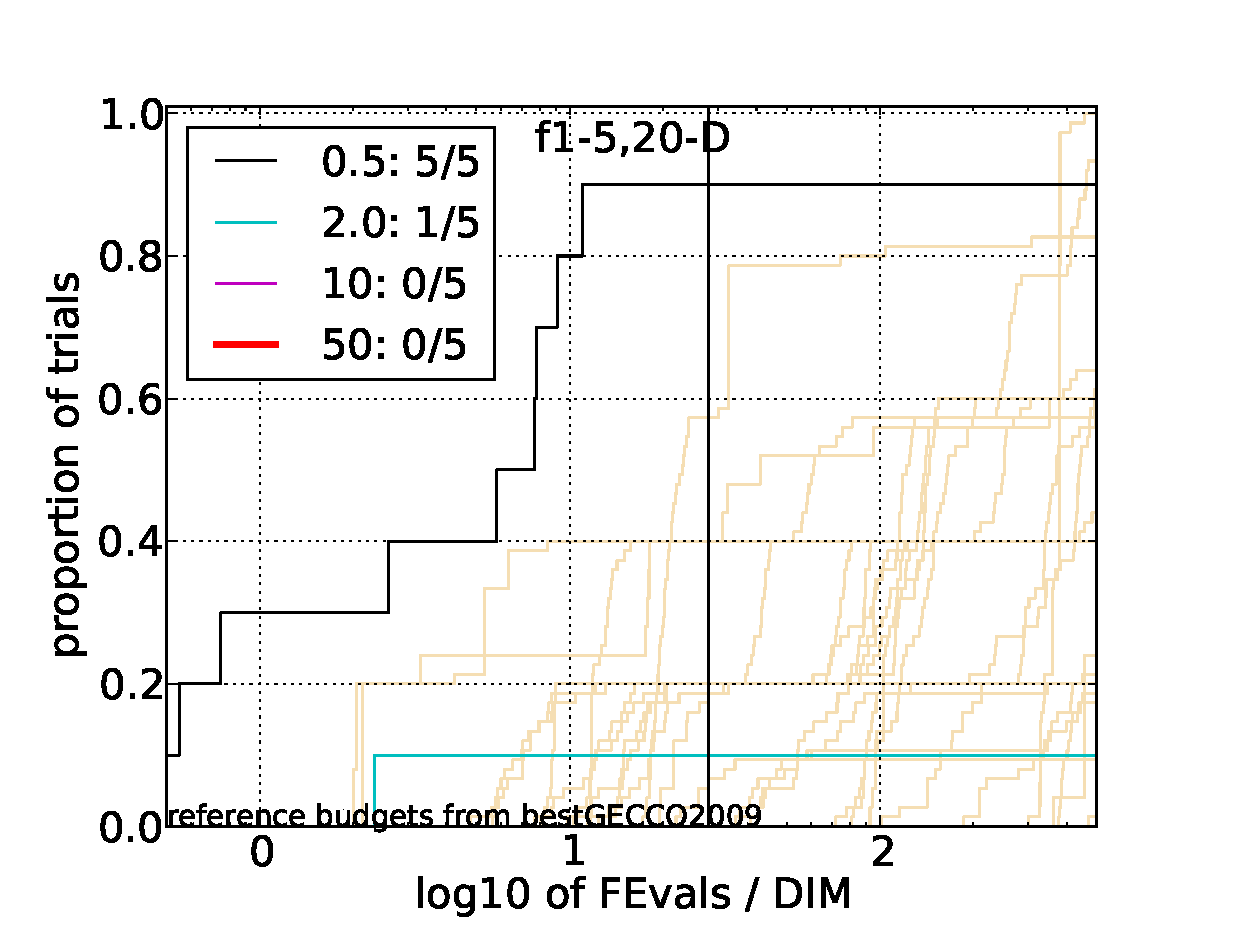
\includegraphics[width=0.268\textwidth,trim=0 0 0 13mm, 
clip]{ppdata_normal/pprldistr_20D_separ} &
\includegraphics[width=0.2362\textwidth,trim=2.40cm 0 0 13mm, 
clip]{ppdata_normal/ppfvdistr_20D_separ} \\[-2ex]
\rot[1]{moderate}
\includegraphics[width=0.268\textwidth,trim=0 0 0 13mm, 
clip]{ppdata_normal/pprldistr_05D_lcond} &
\includegraphics[width=0.2362\textwidth,trim=2.40cm 0 0 13mm, 
clip]{ppdata_normal/ppfvdistr_05D_lcond} &
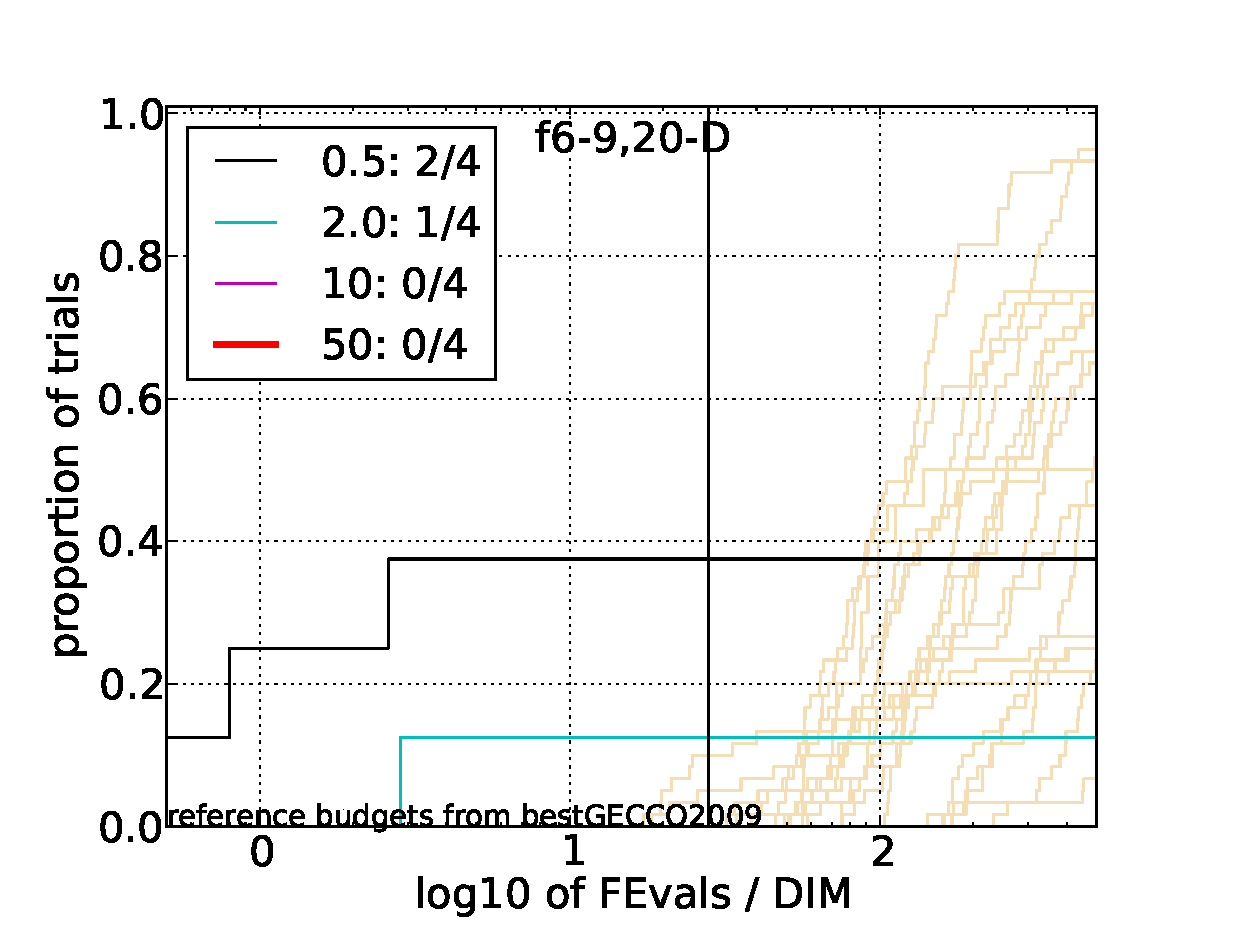
\includegraphics[width=0.268\textwidth,trim=0 0 0 13mm, 
clip]{ppdata_normal/pprldistr_20D_lcond} &
\includegraphics[width=0.2362\textwidth,trim=2.40cm 0 0 13mm, 
clip]{ppdata_normal/ppfvdistr_20D_lcond} \\[-2ex]
\rot[1.3]{ill-cond.}
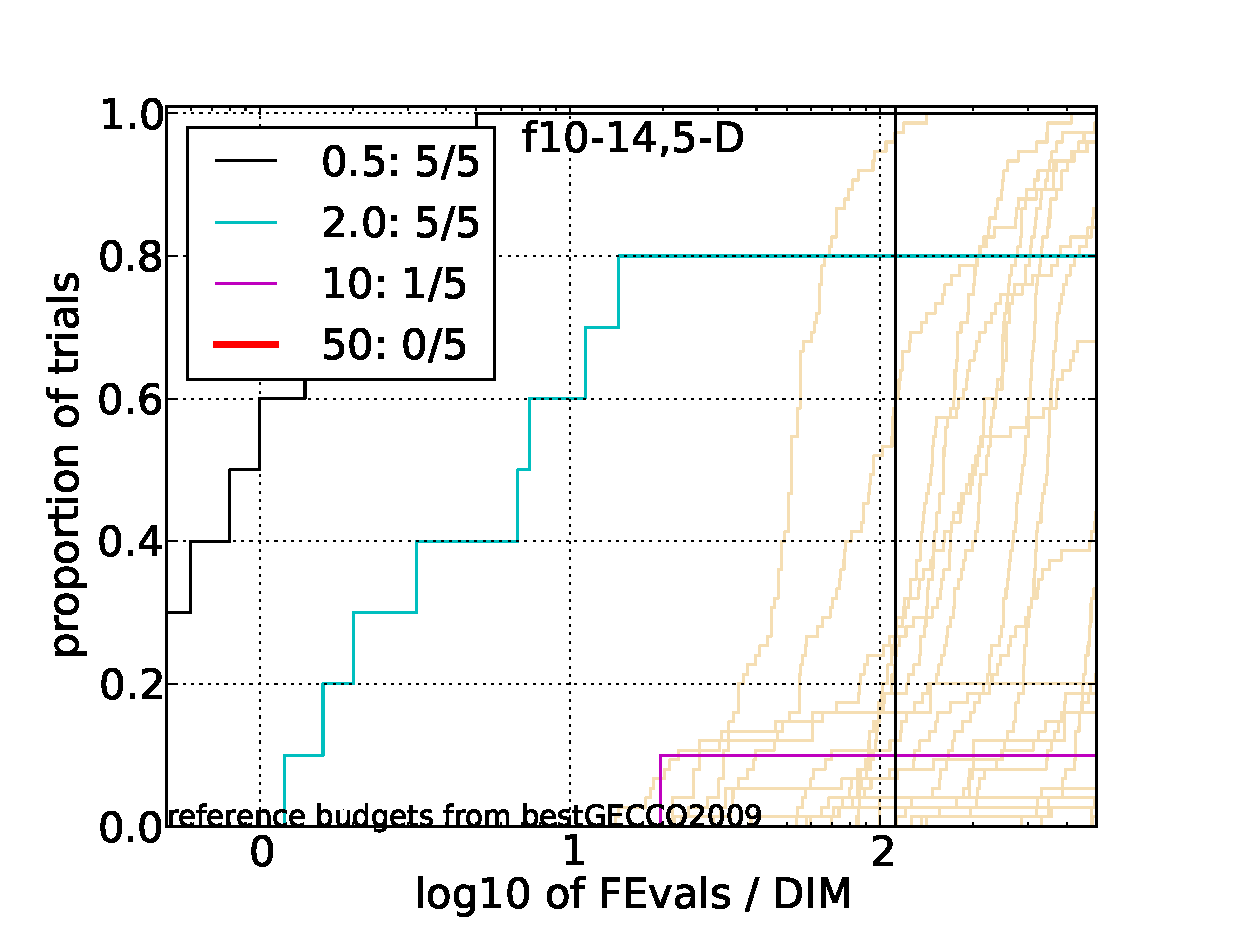
\includegraphics[width=0.268\textwidth,trim=0 0 0 13mm, 
clip]{ppdata_normal/pprldistr_05D_hcond} &
\includegraphics[width=0.2362\textwidth,trim=2.40cm 0 0 13mm, 
clip]{ppdata_normal/ppfvdistr_05D_hcond} &
\includegraphics[width=0.268\textwidth,trim=0 0 0 13mm, 
clip]{ppdata_normal/pprldistr_20D_hcond} &
\includegraphics[width=0.2362\textwidth,trim=2.40cm 0 0 13mm, 
clip]{ppdata_normal/ppfvdistr_20D_hcond} \\[-2ex]
\rot[1.6]{multi-modal}
\includegraphics[width=0.268\textwidth,trim=0 0 0 13mm, 
clip]{ppdata_normal/pprldistr_05D_multi} &
\includegraphics[width=0.2362\textwidth,trim=2.40cm 0 0 13mm, 
clip]{ppdata_normal/ppfvdistr_05D_multi} &
\includegraphics[width=0.268\textwidth,trim=0 0 0 13mm, 
clip]{ppdata_normal/pprldistr_20D_multi} &
\includegraphics[width=0.2362\textwidth,trim=2.40cm 0 0 13mm, 
clip]{ppdata_normal/ppfvdistr_20D_multi} \\[-2ex]
\rot[1.0]{weak struct}
\includegraphics[width=0.268\textwidth,trim=0 0 0 13mm, 
clip]{ppdata_normal/pprldistr_05D_mult2} &
\includegraphics[width=0.2362\textwidth,trim=2.40cm 0 0 13mm, 
clip]{ppdata_normal/ppfvdistr_05D_mult2} &
\includegraphics[width=0.268\textwidth,trim=0 0 0 13mm, 
clip]{ppdata_normal/pprldistr_20D_mult2} &
\includegraphics[width=0.2362\textwidth,trim=2.40cm 0 0 13mm, 
clip]{ppdata_normal/ppfvdistr_20D_mult2}\\[-2ex]
\rot{all}
\includegraphics[width=0.268\textwidth,trim=0 0 0 13mm, 
clip]{ppdata_normal/pprldistr_05D_noiselessall} &
\includegraphics[width=0.2362\textwidth,trim=2.40cm 0 0 13mm, 
clip]{ppdata_normal/ppfvdistr_05D_noiselessall} &
\includegraphics[width=0.268\textwidth,trim=0 0 0 13mm, 
clip]{ppdata_normal/pprldistr_20D_noiselessall} &
\includegraphics[width=0.2362\textwidth,trim=2.40cm 0 0 13mm, 
clip]{ppdata_normal/ppfvdistr_20D_noiselessall}
\vspace*{-0.5ex}
\end{tabular}
\caption{Wykresy ECDF dla rozwiązania z modelem zastępczym (perceptron 
wielowarstwowy z 10 neuronami w warstwie ukrytej).}
\end{figure*}

\begin{comment}
\begin{figure*}
\begin{tabular}{l@{\hspace*{-0.025\textwidth}}l@{\hspace*{-0.00\textwidth}}|l@{
\hspace*{-0.025\textwidth}}l}
\multicolumn{2}{c}{$D=5$} & \multicolumn{2}{c}{$D=20$}\\[-0.5ex]
\rot{separable}
\includegraphics[width=0.268\textwidth,trim=0 0 0 13mm, 
clip]{ppdata_unit50/pprldistr_05D_separ} &
\includegraphics[width=0.2362\textwidth,trim=2.40cm 0 0 13mm, 
clip]{ppdata_unit50/ppfvdistr_05D_separ} &
\includegraphics[width=0.268\textwidth,trim=0 0 0 13mm, 
clip]{ppdata_unit50/pprldistr_20D_separ} &
\includegraphics[width=0.2362\textwidth,trim=2.40cm 0 0 13mm, 
clip]{ppdata_unit50/ppfvdistr_20D_separ} \\[-2ex]
\rot[1]{moderate}
\includegraphics[width=0.268\textwidth,trim=0 0 0 13mm, 
clip]{ppdata_unit50/pprldistr_05D_lcond} &
\includegraphics[width=0.2362\textwidth,trim=2.40cm 0 0 13mm, 
clip]{ppdata_unit50/ppfvdistr_05D_lcond} &
\includegraphics[width=0.268\textwidth,trim=0 0 0 13mm, 
clip]{ppdata_unit50/pprldistr_20D_lcond} &
\includegraphics[width=0.2362\textwidth,trim=2.40cm 0 0 13mm, 
clip]{ppdata_unit50/ppfvdistr_20D_lcond} \\[-2ex]
\rot[1.3]{ill-cond.}
\includegraphics[width=0.268\textwidth,trim=0 0 0 13mm, 
clip]{ppdata_unit50/pprldistr_05D_hcond} &
\includegraphics[width=0.2362\textwidth,trim=2.40cm 0 0 13mm, 
clip]{ppdata_unit50/ppfvdistr_05D_hcond} &
\includegraphics[width=0.268\textwidth,trim=0 0 0 13mm, 
clip]{ppdata_unit50/pprldistr_20D_hcond} &
\includegraphics[width=0.2362\textwidth,trim=2.40cm 0 0 13mm, 
clip]{ppdata_unit50/ppfvdistr_20D_hcond} \\[-2ex]
\rot[1.6]{multi-modal}
\includegraphics[width=0.268\textwidth,trim=0 0 0 13mm, 
clip]{ppdata_unit50/pprldistr_05D_multi} &
\includegraphics[width=0.2362\textwidth,trim=2.40cm 0 0 13mm, 
clip]{ppdata_unit50/ppfvdistr_05D_multi} &
\includegraphics[width=0.268\textwidth,trim=0 0 0 13mm, 
clip]{ppdata_unit50/pprldistr_20D_multi} &
\includegraphics[width=0.2362\textwidth,trim=2.40cm 0 0 13mm, 
clip]{ppdata_unit50/ppfvdistr_20D_multi} \\[-2ex]
\rot[1.0]{weak struct}
\includegraphics[width=0.268\textwidth,trim=0 0 0 13mm, 
clip]{ppdata_unit50/pprldistr_05D_mult2} &
\includegraphics[width=0.2362\textwidth,trim=2.40cm 0 0 13mm, 
clip]{ppdata_unit50/ppfvdistr_05D_mult2} &
\includegraphics[width=0.268\textwidth,trim=0 0 0 13mm, 
clip]{ppdata_unit50/pprldistr_20D_mult2} &
\includegraphics[width=0.2362\textwidth,trim=2.40cm 0 0 13mm, 
clip]{ppdata_unit50/ppfvdistr_20D_mult2}\\[-2ex]
\rot{all}
\includegraphics[width=0.268\textwidth,trim=0 0 0 13mm, 
clip]{ppdata_unit50/pprldistr_05D_noiselessall} &
\includegraphics[width=0.2362\textwidth,trim=2.40cm 0 0 13mm, 
clip]{ppdata_unit50/ppfvdistr_05D_noiselessall} &
\includegraphics[width=0.268\textwidth,trim=0 0 0 13mm, 
clip]{ppdata_unit50/pprldistr_20D_noiselessall} &
\includegraphics[width=0.2362\textwidth,trim=2.40cm 0 0 13mm, 
clip]{ppdata_unit50/ppfvdistr_20D_noiselessall}
\vspace*{-0.5ex}
\end{tabular}
\end{figure*}
\end{comment}
\newpage
\subsection{Algorytm ewolucyjny z wykorzystaniem modelu zastępczego}

Parametry:
\begin{itemize}
 \item rozmiar utrzymywanej populacji $P^t$: $\mu=250$
 \item rozmiar reprodukowanej populacji $O^t$: $\lambda=250$
 \item maksymalna liczba iteracji algorytmu ewolucyjnego: $10000$
 \item liczba neuronów w warstwie ukrytej: $50$
\end{itemize}
\begin{figure*}[!h]
\begin{tabular}{l@{\hspace*{-0.025\textwidth}}l@{\hspace*{-0.00\textwidth}}|l@{
\hspace*{-0.025\textwidth}}l}
\multicolumn{2}{c}{$D=5$} & \multicolumn{2}{c}{$D=20$}\\[-0.5ex]
\rot{separable}
\includegraphics[width=0.268\textwidth,trim=0 0 0 13mm, 
clip]{ppdata_lambda25_mu20/pprldistr_05D_separ} &
\includegraphics[width=0.2362\textwidth,trim=2.40cm 0 0 13mm, 
clip]{ppdata_lambda25_mu20/ppfvdistr_05D_separ} &
\includegraphics[width=0.268\textwidth,trim=0 0 0 13mm, 
clip]{ppdata_lambda25_mu20/pprldistr_20D_separ} &
\includegraphics[width=0.2362\textwidth,trim=2.40cm 0 0 13mm, 
clip]{ppdata_lambda25_mu20/ppfvdistr_20D_separ} \\[-2ex]
\rot[1]{moderate}
\includegraphics[width=0.268\textwidth,trim=0 0 0 13mm, 
clip]{ppdata_lambda25_mu20/pprldistr_05D_lcond} &
\includegraphics[width=0.2362\textwidth,trim=2.40cm 0 0 13mm, 
clip]{ppdata_lambda25_mu20/ppfvdistr_05D_lcond} &
\includegraphics[width=0.268\textwidth,trim=0 0 0 13mm, 
clip]{ppdata_lambda25_mu20/pprldistr_20D_lcond} &
\includegraphics[width=0.2362\textwidth,trim=2.40cm 0 0 13mm, 
clip]{ppdata_lambda25_mu20/ppfvdistr_20D_lcond} \\[-2ex]
\rot[1.3]{ill-cond.}
\includegraphics[width=0.268\textwidth,trim=0 0 0 13mm, 
clip]{ppdata_lambda25_mu20/pprldistr_05D_hcond} &
\includegraphics[width=0.2362\textwidth,trim=2.40cm 0 0 13mm, 
clip]{ppdata_lambda25_mu20/ppfvdistr_05D_hcond} &
\includegraphics[width=0.268\textwidth,trim=0 0 0 13mm, 
clip]{ppdata_lambda25_mu20/pprldistr_20D_hcond} &
\includegraphics[width=0.2362\textwidth,trim=2.40cm 0 0 13mm, 
clip]{ppdata_lambda25_mu20/ppfvdistr_20D_hcond} \\[-2ex]
\rot[1.6]{multi-modal}
\includegraphics[width=0.268\textwidth,trim=0 0 0 13mm, 
clip]{ppdata_lambda25_mu20/pprldistr_05D_multi} &
\includegraphics[width=0.2362\textwidth,trim=2.40cm 0 0 13mm, 
clip]{ppdata_lambda25_mu20/ppfvdistr_05D_multi} &
\includegraphics[width=0.268\textwidth,trim=0 0 0 13mm, 
clip]{ppdata_lambda25_mu20/pprldistr_20D_multi} &
\includegraphics[width=0.2362\textwidth,trim=2.40cm 0 0 13mm, 
clip]{ppdata_lambda25_mu20/ppfvdistr_20D_multi} \\[-2ex]
\rot[1.0]{weak struct}
\includegraphics[width=0.268\textwidth,trim=0 0 0 13mm, 
clip]{ppdata_lambda25_mu20/pprldistr_05D_mult2} &
\includegraphics[width=0.2362\textwidth,trim=2.40cm 0 0 13mm, 
clip]{ppdata_lambda25_mu20/ppfvdistr_05D_mult2} &
\includegraphics[width=0.268\textwidth,trim=0 0 0 13mm, 
clip]{ppdata_lambda25_mu20/pprldistr_20D_mult2} &
\includegraphics[width=0.2362\textwidth,trim=2.40cm 0 0 13mm, 
clip]{ppdata_lambda25_mu20/ppfvdistr_20D_mult2}\\[-2ex]
\rot{all}
\includegraphics[width=0.268\textwidth,trim=0 0 0 13mm, 
clip]{ppdata_lambda25_mu20/pprldistr_05D_noiselessall} &
\includegraphics[width=0.2362\textwidth,trim=2.40cm 0 0 13mm, 
clip]{ppdata_lambda25_mu20/ppfvdistr_05D_noiselessall} &
\includegraphics[width=0.268\textwidth,trim=0 0 0 13mm, 
clip]{ppdata_lambda25_mu20/pprldistr_20D_noiselessall} &
\includegraphics[width=0.2362\textwidth,trim=2.40cm 0 0 13mm, 
clip]{ppdata_lambda25_mu20/ppfvdistr_20D_noiselessall}
\vspace*{-0.5ex}
\end{tabular}
\caption{Wykresy ECDF dla rozwiązania z modelem zastępczym (perceptron 
wielowarstwowy z 50 neuronami w warstwie ukrytej).}
\end{figure*}

\section{Dyskusja wyników}

Dla algorytmu ewolucyjnego, który nie wykorzystuje żadnego modelu zastępczego, 
wymagany minimalny błąd do optimum lokalnego osiągalne 
\section{Wnioski}

Możliwe dobrym rozwiązaniem mogłoby być odpowiednie dobieranie macierzy 
kowariancji rozkładu normalnego, z którego losowane są punkty w trakcie 
eksploatacji.
\begin{thebibliography}{5}
\bibitem{arabas}
Jarosław Arabas, Wykłady z algorytmów ewolucyjnych, Wydawnictwo 
Naukowo-Techniczne Warszawa 2004 
\end{thebibliography}
\end{document}

